\documentclass[12pt,twoside]{article}
\usepackage{geometry}
\usepackage[shortlabels]{enumitem}
\setlist{nosep}
\setlist[enumerate]{wide=0pt, widest=99,leftmargin=25pt, labelsep=*}
\usepackage[none]{hyphenat}
\usepackage{graphicx}
\graphicspath{ {./} }
\usepackage{titlesec}
\usepackage{booktabs}
\usepackage{mathptmx}
\usepackage{setspace}
\setlength{\parindent}{0pt}
\setlength{\parskip}{1em}
\sloppy
\usepackage{array}
\newcolumntype{P}[1]{>{\centering\arraybackslash}p{#1}}
\newcolumntype{M}[1]{>{\centering\arraybackslash}m{#1}}

\titleformat{\section}
  {\normalfont\fontsize{12}{12}\bfseries}{\thesection.}{12pt}{}
\titlespacing*{\section}
  {0pt}{12pt plus 2pt minus 2pt}{0pt}
\titleformat{\subsection}
  {\normalfont\fontsize{12}{12}\bfseries}{\thesubsection}{12pt}{}
\titlespacing*{\subsection}
  {0pt}{10pt plus 2pt minus 2pt}{0pt}

\geometry{a4paper, total={170mm,257mm}, left=2.54cm, top=2.65cm,
          right=2.54cm, bottom=2.65cm}
\rmfamily
\usepackage{fancyhdr}
\renewcommand{\footrulewidth}{0pt}
\renewcommand{\headrulewidth}{0pt}

\begin{document}

\begin{singlespace}
\begin{center}
\fontsize{24}{24}\selectfont\textbf
{Do Adaptive Modality-Acquisition Policies Help? A Cost-Matched Audit of Three Published Methods on ADNI}
\end{center}
\vspace{24pt}
\fontsize{16}{16}\selectfont\textbf{
Rishi Jayanath$^1$}
\vspace{16pt}\\
\fontsize{11}{11}\selectfont {
$^1$[Department], [Institution], [City], [Country]
}\vspace{16pt}\\
{\fontsize{9}{9}\selectfont\textbf{{E-mail:}} $^1$rishi.jayanath@roboticsforyouth.org}\\
\end{singlespace}

\fontsize{12}{12}\selectfont
\begin{onehalfspace}

\section*{Abstract}
Adaptive modality-acquisition policies promise to cut the cost of
Alzheimer's disease prognosis by deciding, per patient, which expensive
scan to order. Several such policies report large reductions in imaging
use at maintained accuracy, but they have not been compared against one
another, nor against the trivial baselines that any cost-saving claim must
beat. This study audits three published policies -- an uncertainty-gated
cascade, a staged evidential method, and a reinforcement-learning test-ordering
policy -- re-implemented under a single leakage-free protocol on 1,622
Alzheimer's Disease Neuroimaging Initiative participants with mild cognitive
impairment at baseline. Policies were evaluated at 12, 24 and 36-month
prediction horizons, under three acquisition-cost regimes, with subject-level
splits and a held-out test set spent once. No policy significantly
outperformed random acquisition at any horizon, and 18 of 33 policy-horizon
pairs were dominated by a patient-independent fixed rule costing no more.
The result survived a predictor swap, a cost-regime sweep, seed variation
and decision-curve analysis. A configuration using established
Alzheimer's-signature structural features reached accuracy statistically
indistinguishable from acquiring four modalities at one-third to one-ninth
of the acquisition cost. Separately, complete-case multimodal analysis is
shown to reduce non-White representation from 17.1\% to 5.9\%, making
race-stratified fairness auditing of conversion models infeasible on current
ADNI data.

\vspace{5pt}
\textbf{\fontsize{12}{12}\selectfont Keywords:} Alzheimer's disease,
modality acquisition, cost-aware machine learning, benchmarking,
algorithmic fairness, mild cognitive impairment

\section{Introduction}
Predicting whether a person with mild cognitive impairment (MCI) will
progress to Alzheimer's disease (AD) dementia is usually framed as a
prediction problem: assemble as many modalities as possible -- structural
MRI, FDG and amyloid PET, cerebrospinal fluid (CSF) assays -- and maximise
discrimination. In a clinic, it is also an economics problem. Amyloid PET
is expensive and exposes the patient to radiation; a lumbar puncture is
invasive; MRI is comparatively cheap. Acquiring everything for everyone is
neither affordable nor necessary.

This has motivated a line of work on \emph{adaptive acquisition policies}:
models that decide, per patient, which modality to acquire next, typically
escalating only the cases the cheaper data leaves uncertain. Published
policies of this kind report substantial savings -- reductions of 50--90\%
in imaging use at maintained accuracy are claimed [1, 2, 3].

These claims have not been tested against each other, and more importantly
they have not been tested against the baselines any cost-saving claim must
clear. Two are essential. The first is \emph{random} acquisition: if
escalating a randomly chosen half of patients performs as well, the policy's
decisions carry no information, only its willingness to spend. The second
is a \emph{fixed} rule that acquires the same modalities for everyone: if a
rule that never looks at the patient matches the policy at equal or lower
cost, personalisation has bought nothing. Neither baseline appears in the
original reports.

This paper supplies that audit. The contributions are:

\begin{enumerate}[(i)]
\item A head-to-head benchmark of three published adaptive acquisition
policies, re-implemented under one leakage-free protocol, across three
prediction horizons and three acquisition-cost regimes, with paired
statistical comparison against random and fixed baselines.
\item A cost-domination analysis quantifying how often a learned policy is
beaten by a patient-independent rule costing no more, and a robustness
sweep over predictor family, cost regime and random seed.
\item A quantification of \emph{representation attrition}: the demographic
cost of the complete-case multimodal designs this literature relies on,
and its consequence for fairness auditing.
\end{enumerate}

We report a largely negative result, and one constructive consequence of
it. We are explicit throughout about which findings are new and which
reproduce established results in a new setting.

\section{Related Work}

\textbf{Adaptive acquisition policies for AD.} Three published methods are
audited here. Zheng et al. [1] gate amyloid-PET acquisition on the
predictive uncertainty of an MRI model, reporting AUC 0.851 with 53.8\% of
patients escalated. A staged evidential method [2] performs Dirichlet-based
evidential classification on cheap clinical data and escalates to MRI or
PET when uncertainty exceeds a learned threshold, fusing modality opinions
by Dempster-Shafer combination and reporting 50--90\% reductions in imaging
use. A reinforcement-learning formulation [3] treats diagnosis as sequential
decision-making, learning a policy that chooses which test to order next.
None of the three reports a comparison against random acquisition or against
a cost-matched fixed rule, and none has been compared against the others.

\textbf{Active feature acquisition.} The broader machine-learning
literature on acquiring features under a budget is mature, with a recent
survey and benchmark [4, 5], and formal evaluation frameworks for the
static and time-varying settings [6]. Our finding is consistent with a
known and uncomfortable pattern in that literature: informed acquisition
strategies frequently fail to beat random selection. This has been
documented as a general result for feature selection [7] and, in a clinical
cohort, as a ``flat-to-negative lift over random'' for acquisition methods
evaluated against clinical labels [8]. Our contribution is not the
discovery of that pattern but its demonstration for these specific,
named AD policies under a controlled protocol.

\textbf{Simple baselines in AD prediction.} That simple models are hard to
beat in this domain is likewise established. The TADPOLE challenge compared
92 algorithms from 33 teams and found that for cognitive-decline forecasting
no submission was considerably better than the organisers' benchmark mixed-effects
model [9]. Our result extends that lesson from forecasting to acquisition.

\textbf{Structural features and incomplete data.} The constructive part of
our result rests on two established findings, and we claim novelty for
neither. First, the AD-signature cortical thickness measure predicts
progression better than hippocampal volume, and performed best among the
MRI and CSF markers compared by Dickerson and Wolk [10]. Second,
restricting analysis to complete cases wastes data: the incomplete-multimodal
learning literature is founded on precisely this observation [11]. What is
new here is the use of these two established techniques as the comparison
baseline against which adaptive policies are measured, which has not
previously been done.

\textbf{Methodological rigour.} Reported accuracies in this field are known
to be inflated by data leakage. A scoping review of 44 AD deep-learning
studies found that 68.2\% relied on ADNI, only 15.9\% performed any external
validation, and that subject-wise rather than slice-wise splitting can move
reported accuracy by 28 percentage points [12, 13]. Our protocol is designed
against these failure modes. Fairness in AD prediction models has been
examined for prediction accuracy [14], but not, to our knowledge, for
acquisition decisions.

\section{Materials and Methods}

\subsection{Cohort}
Data were drawn from ADNI. Diagnosis, demographics, genotype, cognitive
assessments, FreeSurfer morphometry, PET summaries and CSF assays were
assembled from the source tables rather than a pre-merged file. All joins
use ADNI's harmonised visit code; the protocol-specific visit code is not
comparable across study phases and its use silently corrupts longitudinal
merges. Screening visits were coalesced into baseline where no baseline
record exists, with a genuine baseline record always taking precedence --
without this, 294 MCI participants whose diagnosis is recorded only at
screening are dropped, and dropped unevenly by phase.

Inclusion was MCI at the baseline visit, giving 1,622 participants from
3,777. Conversion labels were derived at 12, 24 and 36 months. Participants
with insufficient follow-up are censored and excluded from that horizon's
metrics rather than coded as non-converters; participants reverting to
normal cognition are tracked as a distinct category and never merged into
``stable''. Converter counts were 121, 237 and 297 at the three horizons.

\subsection{Acquirable modality blocks and costs}
Demographics, education, APOE genotype, MMSE and CDR-Sum of Boxes are
treated as always available at zero acquisition cost: they are in hand
before any scan is ordered. Four blocks are acquirable: MRI, FDG-PET,
amyloid-PET and CSF. FDG, amyloid and tau PET are separate scans with
separate tracers and are therefore treated as separate acquisitions rather
than one ``PET'' block; conflating them misstates the decision.

Costs are relative units, not currency, and are deliberately swept across
three regimes rather than fixed: \emph{price-like} (MRI 1.0, FDG 2.0,
amyloid 5.0, CSF 1.5), \emph{flat} (all 1.0, isolating how many tests from
which tests), and \emph{burden} (penalising the invasive lumbar puncture
and radiation-exposing tracers). Any conclusion that holds under only one
regime is reported as regime-dependent.

\subsection{Evaluation protocol}
Comparisons are made on the complete-case cohort for the four blocks, so
that every policy could in principle have acquired anything; otherwise a
policy that happens to prefer the most-available modality wins for the wrong
reason. Splits are at subject level and made before any preprocessing
statistic is computed, stratified jointly on outcome and scanner field
strength. Imputation and scaling are fitted inside each cross-validation
fold on that fold's training rows only. Each policy, including every
internal threshold, is refitted within each fold.

A test set was held out and left untouched through all development, then
spent once. All development figures are five-fold cross-validated on the
remaining subjects.

\subsection{Policies compared}
Reference points are \emph{cheap-only} (never acquires), \emph{acquire-all}
(always acquires everything), \emph{fixed} rules acquiring a set prefix for
every patient, and \emph{random} acquisition at a matched rate. The three
published policies were re-implemented from their descriptions, as no
public code exists for any of them; results should therefore be read as
our implementation of each mechanism rather than a reproduction of the
original numbers.

Prediction is delegated to a shared logistic-regression model bank for all
policies, so that differences between policies are differences in the
\emph{acquisition decision} rather than in predictor strength. For the
evidential method this required an additional variant: its neural predictor
is weaker than logistic regression at this sample size, and reporting only
the faithful version would penalise its decision rule for its predictor.
Both are reported.

\subsection{Statistics}
Differences between policies are assessed by paired bootstrap on pooled
out-of-fold predictions for the same subjects, which is considerably more
sensitive than comparing independent confidence intervals. Acquisition-rate
disparities are tested with a bootstrap over subgroups and corrected for
multiplicity using the Benjamini-Hochberg procedure [15]; with dozens of
(policy, modality) comparisons, uncorrected significance is not evidence.
Calibration is reported as slope, intercept and Brier score, and clinical
utility as net benefit across threshold probabilities [16].

\section{Results and Discussion}

\subsection{No policy outperforms random acquisition}
Table 1 gives cross-validated AUC by policy and horizon on the development
set. Figure 1 plots the same results as a cost-accuracy frontier. The
ordering is stable but the differences are small, and the
statistical comparison is decisive: across all three horizons, \textbf{no
learned policy significantly outperformed random acquisition}. Eleven
policy-horizon pairs were significantly \emph{worse} than random. Only
acquire-all beat random, and only at 36 months.

\begin{center}
\textbf{Table 1.} Cross-validated AUC by policy and horizon (development
set; test set untouched). Cost in relative price-like units.\\\vspace{5pt}
\begin{table}[h]
\begin{center}
\begin{tabular}{|M{5.2cm}|M{1.5cm}|M{1.6cm}|M{1.6cm}|M{1.6cm}|}
\hline
\textbf{Policy} & \textbf{Cost} & \textbf{12 mo} & \textbf{24 mo} & \textbf{36 mo} \\
\hline
cheap-only & 0.00 & 0.817 & 0.824 & 0.796 \\\hline
fixed MRI & 1.00 & 0.836 & 0.870 & 0.849 \\\hline
fixed MRI+FDG & 3.00 & 0.851 & 0.887 & 0.885 \\\hline
uncertainty cascade [1] & 3.63 & 0.852 & 0.886 & 0.865 \\\hline
staged evidential [2] & 4.78 & 0.852 & 0.895 & 0.856 \\\hline
RL test-ordering [3] & 4.81 & 0.849 & 0.866 & 0.882 \\\hline
random acquisition & 5.07 & 0.843 & 0.899 & 0.875 \\\hline
acquire-all & 9.50 & 0.862 & 0.894 & 0.900 \\\hline
\end{tabular}
\end{center}
\end{table}
\end{center}


\begin{center}
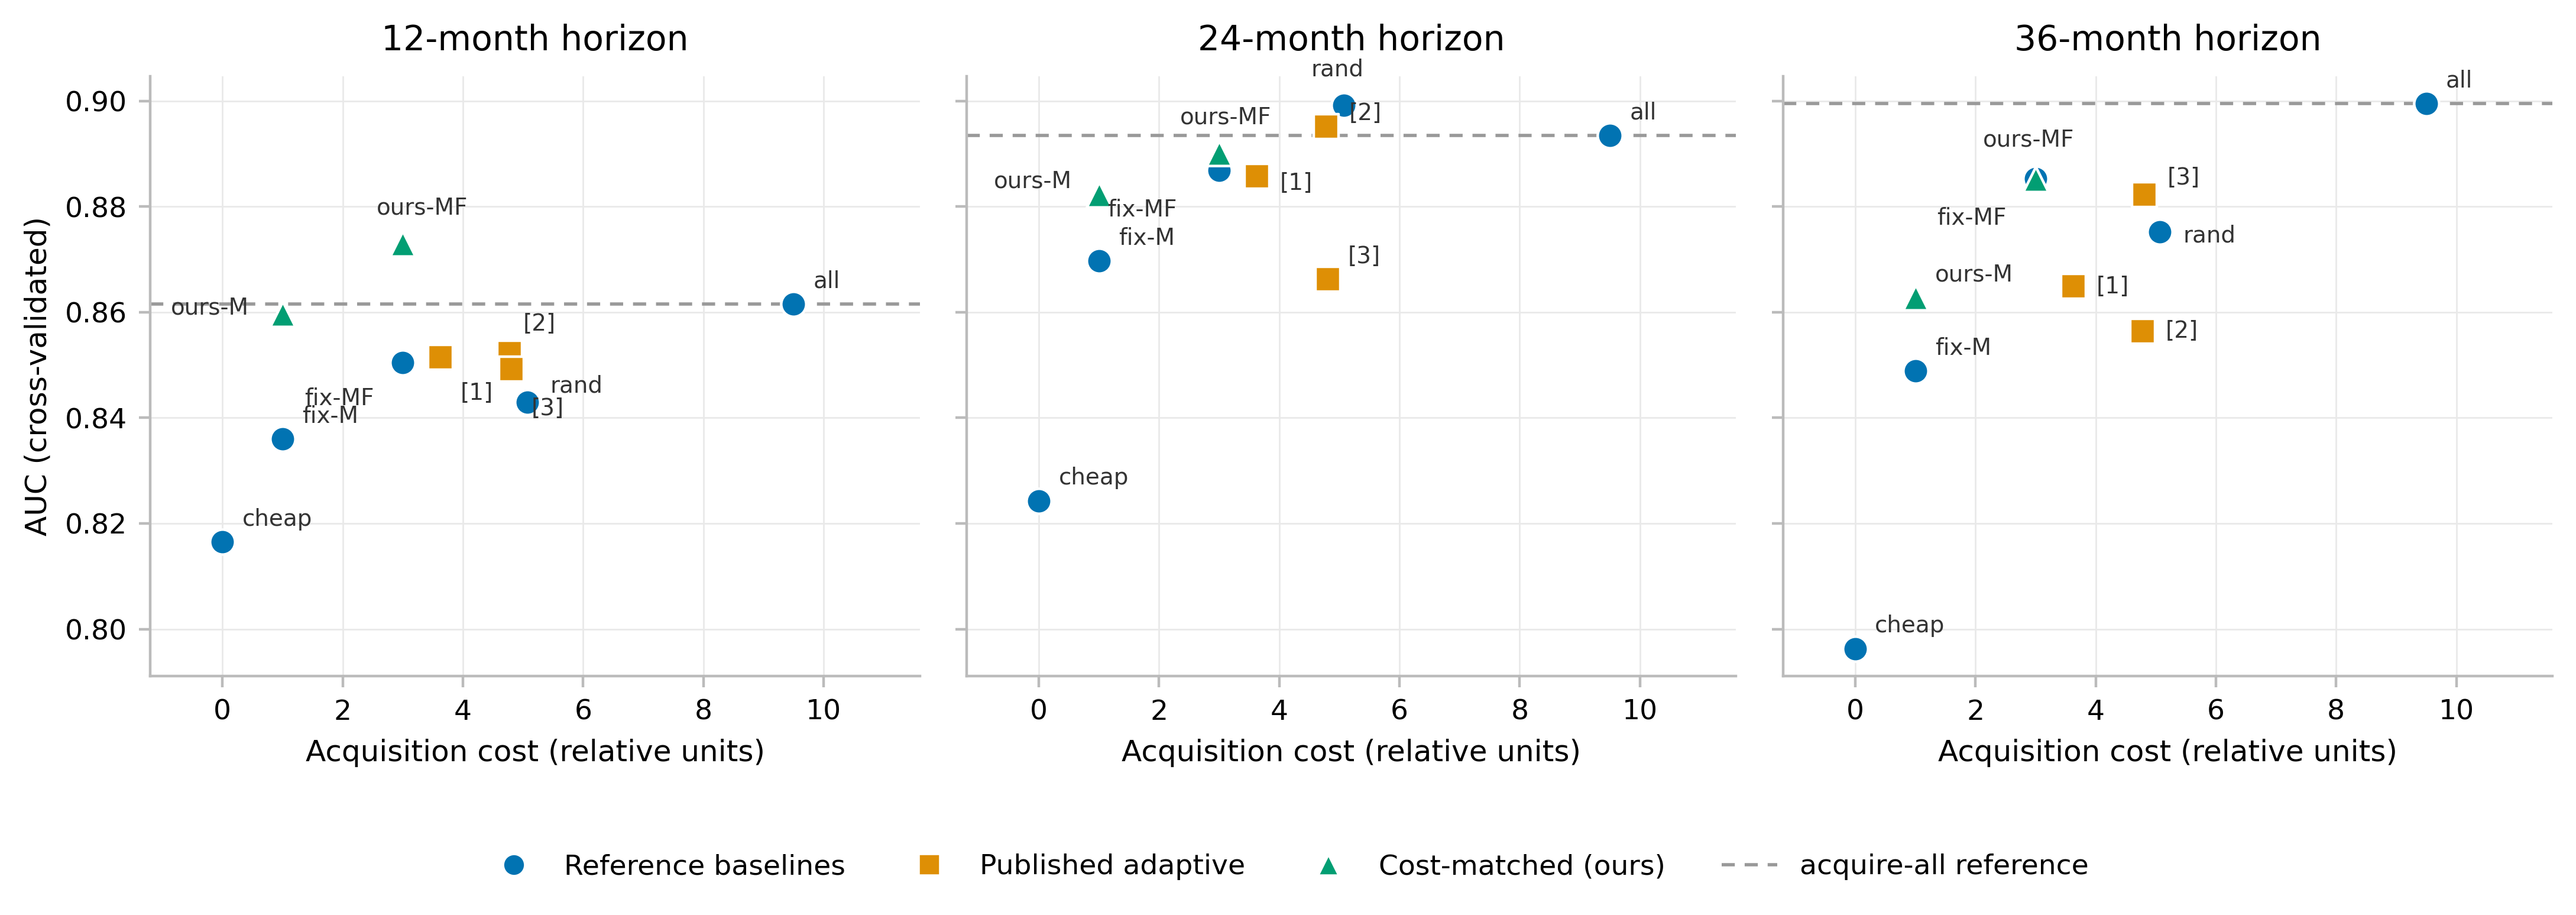
\includegraphics[width=\textwidth]{fig1_cost_accuracy_frontier.png}
\vspace{5pt}
\textbf{Figure 1.} Cost-accuracy frontier at each prediction horizon
(development set, cross-validated). Dashed line marks the accuracy reached
by acquiring all four modalities at cost 9.5. Key: cheap = cheap-only;
fix-M = fixed MRI; fix-MF = fixed MRI+FDG; rand = random acquisition;
all = acquire-all; [1] uncertainty cascade; [2] staged evidential;
[3] RL test-ordering; ours-M and ours-MF = cost-matched configuration.
No published adaptive policy (squares) sits above the reference baselines
(circles) at matched cost.
\vspace{10pt}
\end{center}

\subsection{Learned policies are dominated by fixed rules}
A stronger test than accuracy alone is domination: is a learned policy
beaten by a patient-independent rule that costs no more? Across the three
horizons, \textbf{18 of 33 policy-horizon pairs were dominated}, most often
by ``always acquire MRI+FDG'' (cost 3.00). At 36 months, 9 of 11 learned
configurations were dominated.

This result is cost-regime dependent and we report it as such. Under the
price-like regime the RL policy and the uncertainty cascade are both
dominated; under flat and burden regimes the cascade escapes domination,
and the staged evidential method is dominated under none. The claim that
survives all three regimes is the one in Section 4.1, because a paired
comparison against random makes no cost assumption at all.

\subsection{Robustness}
Three attacks were made on the negative result. Replacing the shared
logistic regression with gradient boosting \emph{strengthened} it: all
three learned policies became dominated, and fixed MRI+FDG reached 0.878
at cost 3.0 against acquire-all's 0.878 at cost 9.5. Varying the random
seed left the ordering unchanged (per-policy SD 0.003--0.011). Decision-curve
analysis extended the finding to clinical utility: across every threshold
probability from 0.05 to 0.50, the best strategy was always random, fixed
or acquire-all, and never a learned policy. Calibration did not favour the
learned policies either -- random acquisition was among the best calibrated
(slope 0.902) and acquire-all the worst (slope 0.686).

\subsection{A cost-matched configuration}
If the savings these policies chase do not require a policy, they should be
obtainable directly. Replacing the customary three-feature MRI block
(hippocampus, ventricles, intracranial volume) with established
AD-signature regions [10], and fitting each acquisition state on every
participant holding that state rather than on complete cases only [11],
yields the configuration in Table 2. Neither ingredient is novel; their use
as the baseline against which adaptive policies are measured is.

\begin{center}
\textbf{Table 2.} Nested cross-validated AUC of the cost-matched
configuration. Nested CV re-selects regularisation within each outer fold;
measured selection optimism was +0.0008 AUC.\\\vspace{5pt}
\begin{table}[h]
\begin{center}
\begin{tabular}{|M{4.4cm}|M{1.5cm}|M{1.6cm}|M{1.6cm}|M{1.6cm}|}
\hline
\textbf{Configuration} & \textbf{Cost} & \textbf{12 mo} & \textbf{24 mo} & \textbf{36 mo} \\
\hline
MRI only & 1.00 & 0.873 & 0.884 & 0.864 \\\hline
MRI + FDG & 3.00 & 0.885 & 0.896 & 0.888 \\\hline
acquire-all (reference) & 9.50 & 0.862 & 0.894 & 0.900 \\\hline
\end{tabular}
\end{center}
\end{table}
\end{center}

On the held-out test set, spent once, the MRI-only configuration reached
AUC 0.947, 0.911 and 0.852 at 12, 24 and 36 months against acquire-all's
0.928, 0.923 and 0.933. Paired against acquire-all, neither configuration
was significantly worse at any horizon. The weakest case is MRI-only at 36
months (--0.081, 95\% CI --0.177 to +0.003), where the interval only just
includes zero; this weakness was visible in development and is reported
rather than rounded away.

Three cautions attach to the test figures. The test sets are small (9, 17
and 22 converters), so ``not significantly worse'' is weak evidence of
equivalence. Test AUCs run above development AUCs by up to 0.074, which is
small-sample variation rather than a real gain -- the nested figures in
Table 2 are the ones to quote as expected performance. And the set was
spent once by design.

\subsection{Representation attrition and the limits of fairness auditing}
The complete-case multimodal design this literature relies on has a
demographic cost that is not usually reported. Table 3 traces it.

\begin{center}
\textbf{Table 3.} Representation attrition through cohort construction
(24-month horizon).\\\vspace{5pt}
\begin{table}[h]
\begin{center}
\begin{tabular}{|M{6.2cm}|M{1.6cm}|M{2.4cm}|M{2.4cm}|}
\hline
\textbf{Stage} & \textbf{n} & \textbf{non-White (n)} & \textbf{non-White (\%)} \\
\hline
MCI at baseline & 1622 & 277 & 17.1 \\\hline
+ has 24-month outcome & 904 & 69 & 7.6 \\\hline
+ complete four modalities & 457 & 27 & 5.9 \\\hline
\end{tabular}
\end{center}
\end{table}
\end{center}

Requiring an outcome label removes three-quarters of non-White
participants, and requiring complete modalities removes most of the
remainder. The mechanism is identifiable: ADNI's most recent phase is
49.8\% non-White, a substantial recruitment improvement, but only 1.7\% of
its participants yet have 24-month follow-up. ADNI's diversity gains are
therefore structurally invisible to conversion-prediction studies at
present.

The practical consequence is that a race-stratified fairness audit of these
policies is not currently feasible: the audit cohort contains 10 Black and
8 Hispanic participants with no converters between them. On sex, the only
adequately powered dimension, no acquisition disparity survived
multiplicity correction. Two gaps were significant uncorrected -- the RL
policy sending one sex for FDG-PET 11.1 percentage points more often
($p=0.011$) and the evidential method 11.2 points less often ($p=0.029$) --
but neither survived Benjamini-Hochberg across the comparison family, and
they are reported as suggestive only. We note that fixed policies cannot
exhibit acquisition disparity at all, since they do not consult the
patient.

\subsection{Horizon dependence}
A secondary analysis asked whether modality value depends on the prediction
horizon, which would motivate horizon-conditioned policies. On a fixed
subject set, only amyloid-PET showed a significant increase in incremental
value from 12 to 36 months (+0.054, 95\% CI +0.014 to +0.095); MRI, FDG and
CSF did not. A horizon-conditioned policy built on this effect did not
outperform horizon-swapped controls, indicating the effect is real as a
measurement but not exploitable as an acquisition rule at this sample size.

\subsection{Limitations}
The three policies are re-implementations from published descriptions, as
no public code exists for any of them; a negative result about a
re-implementation is weaker evidence than one about original code, and we
state this plainly. Sample sizes are modest -- 67 converters in the
24-month development cohort and 17 in its test set -- so several
non-significant comparisons are underpowered, and ``not distinguishable''
should not be read as ``equivalent''. Acquisition costs are relative units
whose absolute values are contestable, which is why every cost-dependent
conclusion is reported across three regimes. ADNI's missingness is
protocol-driven rather than random, so any retrospective estimate of what
could have been skipped is a simulation and not a prospective guarantee.
MRI morphometry pools several FreeSurfer pipeline versions, and the results
come from a single cohort without external validation.

\section{Conclusion}
Three published adaptive modality-acquisition policies for Alzheimer's
disease prognosis were re-implemented and audited under a common
leakage-free protocol across three prediction horizons and three cost
regimes. None significantly outperformed random acquisition at any horizon,
18 of 33 policy-horizon pairs were dominated by a patient-independent fixed
rule costing no more, and the finding survived a predictor swap, a seed
sweep and decision-curve analysis. The cost savings these methods report
are real, but they do not appear to derive from personalisation: a rule
that ignores the patient entirely captures them as well.

Consistent with this, a configuration built from two established techniques
-- AD-signature structural features and training on partially observed
participants -- reached accuracy statistically indistinguishable from
acquiring four modalities at one-third to one-ninth of the acquisition
cost, with the caveat that its cheapest operating point weakens at the
36-month horizon.

Finally, complete-case multimodal analysis reduces non-White representation
in this cohort from 17.1\% to 5.9\%, and recent recruitment gains are not
yet visible to conversion studies because those participants lack
follow-up. Race-stratified fairness auditing of acquisition policies on
ADNI is therefore not currently feasible, a constraint the field should
state explicitly rather than rediscover per study.

Future work should test these policies on prospective or more diverse
cohorts, and should evaluate acquisition methods against random and
cost-matched fixed baselines as a default, since neither appears in the
original reports.

\section*{\fontsize{12}{12}\selectfont\textbf{Funding Statement}}
This research received no specific grant from any funding agency in the
public, commercial, or not-for-profit sectors.

\section*{\fontsize{12}{12}\selectfont\textbf{Ethical Statement}}
This study is a secondary analysis of de-identified data obtained from the
Alzheimer's Disease Neuroimaging Initiative (ADNI). Ethical approval and
participant informed consent were obtained by the ADNI investigators at
each participating site. No new human-subject data were collected and no
identifiable participant information was accessed. Data were used in
accordance with the ADNI Data Use Agreement.

\section*{\fontsize{12}{12}\selectfont\textbf{Conflicts of Interest}}
The author declares no conflicts of interest.

\section*{\fontsize{12}{12}\selectfont\textbf{Acknowledgement}}
Data used in preparation of this article were obtained from the Alzheimer's
Disease Neuroimaging Initiative (ADNI) database (adni.loni.usc.edu). As
such, the investigators within the ADNI contributed to the design and
implementation of ADNI and/or provided data but did not participate in
analysis or writing of this report. A complete listing of ADNI
investigators can be found at:
http://adni.loni.usc.edu/wp-content/uploads/how\_to\_apply/ADNI\_Acknowledgement\_List.pdf

\section*{\fontsize{12}{12}\selectfont\textbf{References}}
\begin{enumerate}[{[1]}]
\item Zheng, B., Chen, X., \& Ye, Y. (2023). Uncertainty-driven modality selection for data-efficient prediction of Alzheimer's disease. \textit{IISE Transactions on Healthcare Systems Engineering, 14}(1). https://doi.org/10.1080/24725579.2023.2227197
\item ProMUSE: Progressive multi-modal uncertainty-guided staged evidential Alzheimer disease classification. (2026). \textit{arXiv preprint} arXiv:2606.19371.
\item Efficient Alzheimer's diagnosis through sequential decision-making with reinforcement learning. (2025). In \textit{Proceedings of the 2025 7th International Conference on Big-Data Service and Intelligent Computation}. https://doi.org/10.1145/3778265.3778280
\item Aronsson, L., Rahbar, A., \& Chehreghani, M. H. (2025). A survey on active feature acquisition strategies. \textit{arXiv preprint}.
\item Schutz, V., Wu, H., Rezvan, R., Aronsson, L., \& Chehreghani, M. H. (2025). AFABench: A generic framework for benchmarking active feature acquisition. \textit{arXiv preprint}.
\item von Kleist, H., Zamanian, A., Shpitser, I., \& Ahmidi, N. (2023). Evaluation of active feature acquisition methods for static feature settings. \textit{arXiv preprint} arXiv:2312.03619.
\item Worse than random: The importance of a baseline for unsupervised feature selection. (2026). \textit{arXiv preprint} arXiv:2605.22973.
\item Perets, B., Mendelson, N., Vainberg, S., Chowers, Y., Shen-Orr, S., \& Mannor, S. (2026). Zero-shot active feature acquisition via LLM-elicitation. \textit{arXiv preprint} arXiv:2606.18933.
\item Marinescu, R. V., Oxtoby, N. P., Young, A. L., Bron, E. E., Toga, A. W., Weiner, M. W., \& Alexander, D. C. (2020). TADPOLE Challenge: Accurate Alzheimer's disease prediction through crowdsourced forecasting of future data. \textit{arXiv preprint} arXiv:2001.09016.
\item Dickerson, B. C., \& Wolk, D. A. (2013). Biomarker-based prediction of progression in MCI: Comparison of AD signature and hippocampal volume with spinal fluid amyloid-beta and tau. \textit{Frontiers in Aging Neuroscience, 5}, 55. https://doi.org/10.3389/fnagi.2013.00055
\item Liu, M., Gao, Y., Yap, P.-T., \& Shen, D. (2017). Multi-stage diagnosis of Alzheimer's disease with incomplete multimodal data via multi-task deep learning. \textit{Deep Learning in Medical Image Analysis}, 1--9.
\item Young, V. M., Gates, S., Garcia, L. Y., \& Salardini, A. (2025). Data leakage in deep learning for Alzheimer's disease diagnosis: A scoping review of methodological rigor and performance inflation. \textit{Diagnostics, 15}(18), 2348. https://doi.org/10.3390/diagnostics15182348
\item Wen, J., Thibeau-Sutre, E., Diaz-Melo, M., Samper-Gonzalez, J., Routier, A., Bottani, S., \& Colliot, O. (2020). Convolutional neural networks for classification of Alzheimer's disease: Overview and reproducible evaluation. \textit{Medical Image Analysis, 63}, 101694. https://doi.org/10.1016/j.media.2020.101694
\item Yuan, C., Linn, K. A., \& Hubbard, R. A. (2023). Algorithmic fairness of machine learning models for Alzheimer disease progression. \textit{JAMA Network Open, 6}(11), e2342203.
\item Benjamini, Y., \& Hochberg, Y. (1995). Controlling the false discovery rate: A practical and powerful approach to multiple testing. \textit{Journal of the Royal Statistical Society: Series B, 57}(1), 289--300.
\item Vickers, A. J., \& Elkin, E. B. (2006). Decision curve analysis: A novel method for evaluating prediction models. \textit{Medical Decision Making, 26}(6), 565--574.
\item Sensoy, M., Kaplan, L., \& Kandemir, M. (2018). Evidential deep learning to quantify classification uncertainty. In \textit{Advances in Neural Information Processing Systems, 31}.
\end{enumerate}

\section*{\fontsize{12}{12}\selectfont\textbf{Author's biography}}
\textbf{Rishi Jayanath} [Author biography of up to 200 words, with photograph, to be supplied.]

\end{onehalfspace}
\end{document}
